\documentclass[11pt,a4paper]{article}
\usepackage{amsmath}
\usepackage{amsfonts}
\usepackage{amssymb}
\usepackage{makeidx}
\usepackage{graphicx}
\usepackage{wrapfig}
\usepackage{enumerate}
\usepackage{pdfpages}
\usepackage{tocloft}
\usepackage{setspace}
\usepackage{mathtools}
\usepackage{hyperref}
\definecolor{linkcolour}{rgb}{0,0.2,0.6} % Link color
\hypersetup{colorlinks,breaklinks,urlcolor=linkcolour,linkcolor=linkcolour}

\usepackage[left=2cm,right=2cm,top=1.5cm,bottom=1.5cm]{geometry}

\usepackage{xcolor}

\usepackage{color,soul}
\usepackage{fontspec}
\setmainfont{Cambria}

\usepackage{caption}
\captionsetup[figure]{font=small, labelfont={bf}}
\captionsetup[table]{font=small, labelfont={bf}}

\usepackage{float}
\usepackage{multirow}
\usepackage{longtable}

\usepackage[nottoc]{tocbibind}

\newcommand{\spa}{\vspace{1.25em}}
\newcommand{\noi}{\noindent}
\def\dul#1{\underline{\underline{#1}}}
\def\cpt#1#2{{\begin{center}\small\textbf{\textcolor{blue}{Figure #1:}} #2\end{center}}}
\def\tt#1{\texttt{#1}}
\def\colortt#1{\textcolor{blue}{\texttt{#1}}}

% for dots in the content
\usepackage{tocloft}
\renewcommand{\cftsecleader}{\cftdotfill{\cftdotsep}}

\begin{document}
	\begin{titlepage} 
		\begin{center}
		\large{ASSIGNMENT 3}\\
		\vspace{2em}
		\large {CS5691 Pattern Recognition and Machine Learning}
		\vspace{3em}
		
		\rule{0.9\linewidth}{0.5mm} \\[0.4cm]
	    {\Large{\bfseries{CS5691 Assignment 3}}} \\
	    \rule{0.9\linewidth}{0.5mm} \\[3 em]	
	    
	    Team Members: \\
	    \vspace{0.5em}
	   	\def\arraystretch{1.25}
\begin{tabular}{c l}
	\hline
	BE17B007 & N Sowmya Manojna \\
	PH17B010 & Thakkar Riya Anandbhai \\
	PH17B011 & Chaithanya Krishna Moorthy \\
	\hline
\end{tabular}

		\vspace{1em}

		Indian Institute of Technology, Madras\\    
		
		\vspace{5em}    
	    
	    	
\includegraphics[scale = 0.09]{images/iitmlogo.png}
		\end{center}
	\end{titlepage}

{\hypersetup{linkcolor=black}
 \tableofcontents}
\break


%%%%%%%%%%%%%%%%%%%%%%%%%%%%%%%%%%%%%%%%%%%%%%%
%%%%%%%%%%%%%%%%%%%%%%%%%%%%%%%%%%%%%%%%%%%%%%%
\section{Dataset 1A}
%%%%%%%%%%%%%%%%%%%%%%%%%%%%%%%%%%%%%%%%%%%%%%%
%%%%%%%%%%%%%%%%%%%%%%%%%%%%%%%%%%%%%%%%%%%%%%%
\subsection{Perceptron}


%%%%%%%%%%%%%%%%%%%%%%%%%%%%%%%%%%%%%%%%%%%%%%%
\subsection{MLFFNN}
The classification accuracies on the training and validation datasets are as follows:
\def\arraystretch{1.25}
\begin{center}
{\small
\begin{tabular}{l l l l l l l c}
\hline
\hline
\textbf{\# Neurons} & \textbf{Activation} & \textbf{Solver} & \textbf{Batch Size} & \textbf{\alpha} & \textbf{Learning Rate} & \textbf{Accuracy} & \textbf{Validation Accuracy} \\
\hline
\hline
5 & tanh & lbfgs & 200 & 0.0001 & adaptive & 100.0 & 100.0 \\
5 & tanh & lbfgs & 200 & 0.0001 & constant & 100.0 & 100.0 \\
5 & tanh & lbfgs & 200 & 0.0 & invscaling & 100.0 & 100.0 \\
5 & tanh & lbfgs & 200 & 0.0 & adaptive & 100.0 & 100.0 \\
5 & tanh & lbfgs & 200 & 0.0 & constant & 100.0 & 100.0 \\
5 & tanh & lbfgs & 100 & 0.0 & adaptive & 100.0 & 100.0 \\
5 & tanh & lbfgs & 100 & 0.0001 & invscaling & 100.0 & 100.0 \\
5 & relu & lbfgs & 200 & 0.0 & constant & 100.0 & 100.0 \\
5 & relu & lbfgs & 100 & 0.0001 & invscaling & 100.0 & 100.0 \\
5 & relu & lbfgs & 200 & 0.0 & adaptive & 100.0 & 100.0 \\
\hline
\end{tabular}
\setcounter{table}{1}
\captionof{table}{Best 10 Train and Validation Accuracies obtained after performing a \colortt{GridSearch} on 432 parameter combinations.}
}
\end{center}

\noi
In addition, the parameter combination were sorted based on minimum fitting time (least fitting time - first) and the model that gave the best accuracy the fastest was chosen. Hence the best parameter combination chosen is:
\begin{itemize}
    \itemsep0em
    \item hidden\_layer\_sizes: 5
    \item activation: tanh
    \item solver: lbfgs
    \item batch\_size: 200
    \item alpha: 0.0001
    \item learning\_rate: adaptive
\end{itemize}

\noi
The classification accuracy of the best model on the testing data is: $100\%$. The confusion matrices obtained are as follows:
\begin{figure}[H]
    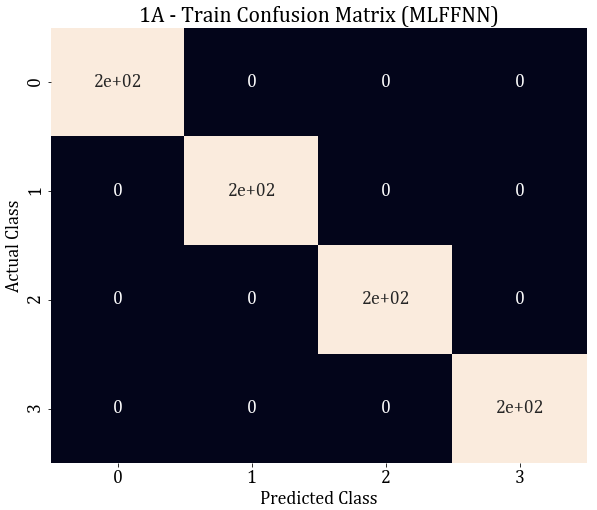
\includegraphics[scale=0.4]{images/1A_MLFFNN_train_confmat.png}
    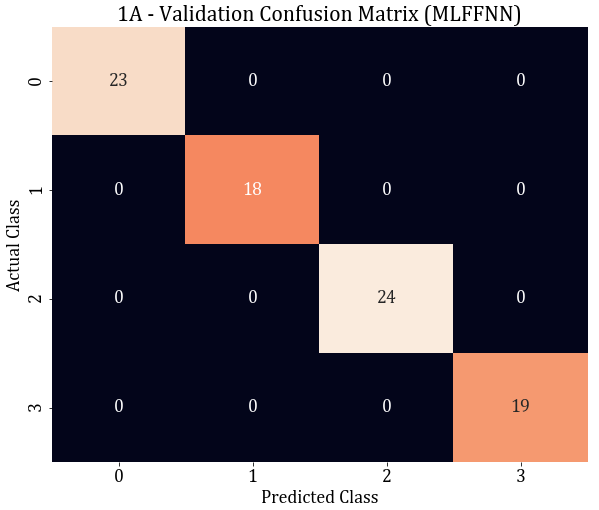
\includegraphics[scale=0.4]{images/1A_MLFFNN_val_confmat.png}
    \caption{Training and Validation confusion matrices obtained for the best parameter combination, on the left and right respectively.}
\end{figure}

\begin{figure}[H]
    \centering
    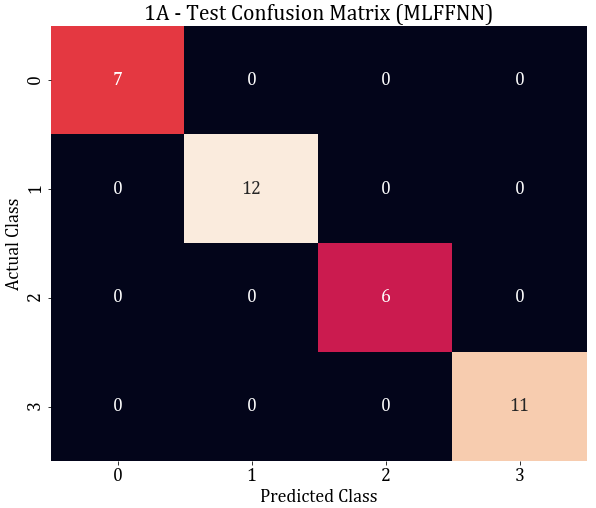
\includegraphics[scale=0.4]{images/1A_MLFFNN_test_confmat.png}
    \caption{Testing confusion matrices obtained for the best parameter combination.}
\end{figure}

\noi
The decision region plots obtained is as follows:
\begin{figure}[H]
    \centering
    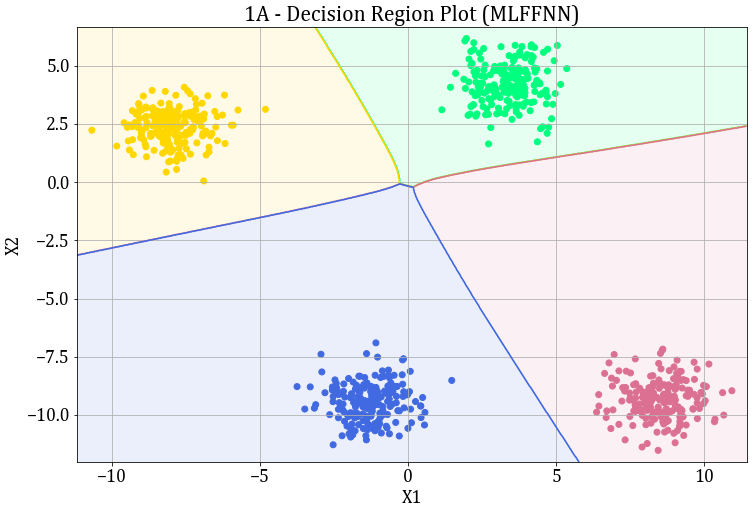
\includegraphics[scale=0.6]{images/1A_MLFFNN_Decision_Plot.png}
    \caption{Decision Region Plot obtained for the best parameter combination.}
\end{figure}

%%%%%%%%%%%%%%%%%%%%%%%%%%%%%%%%%%%%%%%%%%%%%%%
\subsection{Linear SVM}

\break
%%%%%%%%%%%%%%%%%%%%%%%%%%%%%%%%%%%%%%%%%%%%%%%
%%%%%%%%%%%%%%%%%%%%%%%%%%%%%%%%%%%%%%%%%%%%%%%
\section{Dataset 1B}
%%%%%%%%%%%%%%%%%%%%%%%%%%%%%%%%%%%%%%%%%%%%%%%
%%%%%%%%%%%%%%%%%%%%%%%%%%%%%%%%%%%%%%%%%%%%%%%
\subsection{MLFFNN}
The classification accuracies on the training and validation datasets are as follows:
\def\arraystretch{1.25}
\begin{center}
{\small
\begin{tabular}{l l l l l l c c}
\hline
\hline
\textbf{\# Neurons} & \textbf{Activation} & \textbf{Batch Size} & \textbf{Early Stopping} & \textbf{Learning Rate} & \textbf{\alpha} & \textbf{Accuracy} & \textbf{Validation Accuracy} \\
\hline
\hline
(8, 8) & relu & 50 & False & adaptive & 0.01 & 99.33 & 98.41  \\
(8, 8) & relu & 50 & False & constant & 0.001 & 99.33 & 98.41  \\
(8, 8) & relu & 50 & False & invscaling & 0.01 & 99.33 & 98.41  \\
(8, 8) & relu & 50 & False & adaptive & 0.001 & 99.33 & 98.41  \\
(8, 8) & relu & 50 & False & invscaling & 0.001 & 99.33 & 98.41  \\
(8, 8) & relu & 50 & False & constant & 0.01 & 99.33 & 98.41  \\
(10, 10) & relu & 50 & False & adaptive & 0.01 & 99.0 & 98.41  \\
(10, 10) & relu & 50 & False & constant & 0.01 & 99.0 & 98.41  \\
(10, 10) & relu & 50 & False & invscaling & 0.01 & 99.0 & 98.41  \\
(10, 10) & relu & 50 & False & constant & 0.001 & 99.0 & 96.82  \\
\hline
\end{tabular}
\captionof{table}{Best 10 Train and Validation Accuracies obtained after performing a \colortt{GridSearch} on 432 parameter combinations.}
}
\end{center}

\noi
In addition, the parameter combination were sorted based on minimum fitting time (least fitting time - first) and the model that gave the best accuracy the fastest was chosen. Hence the best parameter combination chosen is:
\begin{itemize}
    \itemsep0em
    \item hidden\_layer\_sizes: (8, 8)
    \item activation: relu
    \item batch\_size: 50
    \item early\_stopping: False
    \item learning\_rate: adaptive
    \item alpha: 0.01
\end{itemize}

\noi
The classification accuracy of the best model on the testing data is: $96.296\%$. The confusion matrices obtained are as follows:
\begin{figure}[H]
    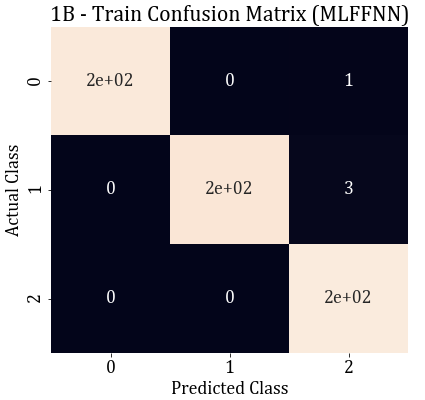
\includegraphics[scale=0.4]{images/1B_MLFFNN_train_confmat.png}
    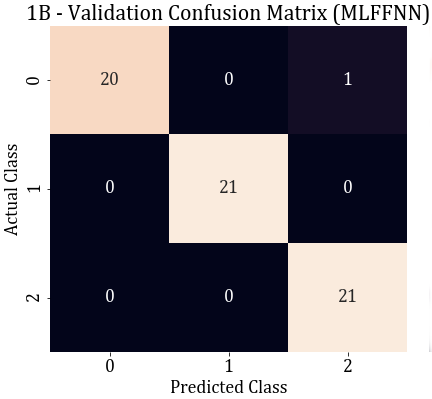
\includegraphics[scale=0.4]{images/1B_MLFFNN_val_confmat.png}
    \caption{Training and Validation confusion matrices obtained for the best parameter combination, on the left and right respectively.}
\end{figure}

\begin{figure}[H]
    \centering
    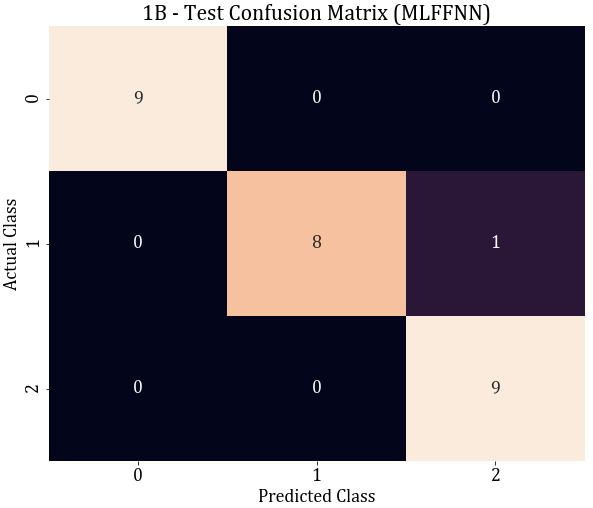
\includegraphics[scale=0.4]{images/1B_MLFFNN_test_confmat.png}
    \caption{Testing confusion matrices obtained for the best parameter combination.}
\end{figure}

\noi
The decision region plots obtained is as follows:
\begin{figure}[H]
    \centering
    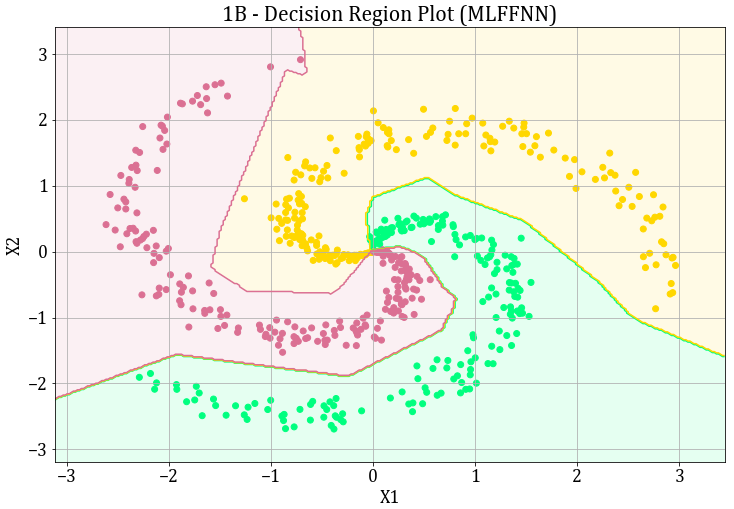
\includegraphics[scale=0.6]{images/1B_MLFFNN_Decision_Plot.png}
    \caption{Decision Region Plot obtained for the best parameter combination.}
\end{figure}
%%%%%%%%%%%%%%%%%%%%%%%%%%%%%%%%%%%%%%%%%%%%%%%
\subsection{Non-Linear SVM}

%%%%%%%%%%%%%%%%%%%%%%%%%%%%%%%%%%%%%%%%%%%%%%%
\break
%%%%%%%%%%%%%%%%%%%%%%%%%%%%%%%%%%%%%%%%%%%%%%%
\section{Dataset 2A}
%%%%%%%%%%%%%%%%%%%%%%%%%%%%%%%%%%%%%%%%%%%%%%%
%%%%%%%%%%%%%%%%%%%%%%%%%%%%%%%%%%%%%%%%%%%%%%%
\subsection{MLFFNN}
%%%%%%%%%%%%%%%%%%%%%%%%%%%%%%%%%%%%%%%%%%%%%%%
\subsection{Gaussian-kernel SVM}

\end{document}
